\subsection{RQ1: Is code-coverage an efficient guide for generating diverse traffic scenarios?}

The main goal of this paper is to increase the diversity of scenarios encountered by an AV while navigating scenarios.
% 
Our primary hypothesis is that code-coverage is not an optimal feedback for guiding a fuzzer for this purpose.
%
The rationale 
%
This is important because off-the-shelf fuzzers use code-coverage for feedback and don't support user-defined coverage criteria.
%
To support our hypothesis, we develop our own fuzzer to show that improvement in test-case diversity can be achieved by using a more appropriate feedback.
%
We hope that our results encourage development of more flexible fuzzers to expand the reach and utility of this successful search technique.


%---------------------
\subsubsection{Performance Metrics}
We use two different metrics to compare our fuzzing technique with the baselines.
%
First, we use the total number of predicate valuations found per wall-clock time.
%
A predicate valuation can be represented as the set of predicates that evaluate to True.
%
Second, we use the total number of predicate-sets found per valid fuzz inputs found per wall-clock time.
%
The motivation behind the second metric is that test-case execution is expensive, so it's better to achieve the same coverage with less number of inputs.
%
This is the same idea behind \emph{corpus minimization} in fuzzing.
%
Nevertheless, the first metric is more important than the second one.


%---------------------
\subsubsection{Baselines}
The first baseline is a random fuzzer.
%
That is, at each fuzzing step, a fuzz-candidate is selected uniformly randomly.
%
The selected candidate is then mutated with the structure-aware mutators and then passed to input evaluation.


The second baseline, \emph{Atheris}, is a code-coverage-guided fuzzer.
%
Atheris supports fuzzing python programs, and is based on libfuzzer under the hood.
%
We configure Atheris to use our structure-aware mutators.
%
Libfuzzer, and so Atheris, use the Entropic power schedule.


%---------------------
\subsubsection{Our Fuzzer}
Our fuzzer uses the structure-aware mutators, similar to the baselines.
%
It also uses the Entropic power schedule, similar to Atheris.
%
We implemented Entropic in python by translating libfuzzer's C++ source code.
%
However, our Entropic implementation does not consider the size of fuzz-inputs, so it does not replace a fuzz-candidate with a smaller new one that has the same coverage.
%
Our fuzzer uses predicate-set coverage feedback to decide whether to add a mutant to the fuzz-candidates, and for calculating the energy of the fuzz-candidates.
%
In the following we refer to this fuzzer as PCGF-Entropic, for Predicate-Coverage-Guided-Fuzzer with the Entropic power schedule.


%---------------------
\subsubsection{Trials}
We compare our fuzzer against the baselines for four different ego agents.
%
For each choice of ego agent, the experiment is repeated for 10 trials, each trial with a different PRNG seed from the set $\{ 0, \dots, 9 \}$.
%
We chose the following agents since they are all compatible with our SCENIC-CARLA simulation platform:
\begin{itemize}
    \item TF++.
        Trans-Fuser Plus Plus \cite{Jaeger.2023} is one of the top agents in CARLA Leaderboard 2.0.
        %
        We run the SENSORS Track version of the agent.
    \item CARLA Autopilot.
        This is a privileged agent controlled by CARLA's traffic manager.
    \item CARLA BehaviorAgent.
        This is a rule-based agent example provided by CARLA which demonstrates how to use CARLA's interface to implement custom agents.
    \item SCENIC agent.
        This is a rule-based agent implemented in the SCENIC language.
        %
        This agent is run using SCENIC's built-in NewtonianSimulator which only simulates the dynamics of vehicles based on a bicycle model.
        %
        The agent is controlled by SCENIC's path-following PID controllers for lateral and longitudinal control.
\end{itemize}


\begin{figure}
    \centering
    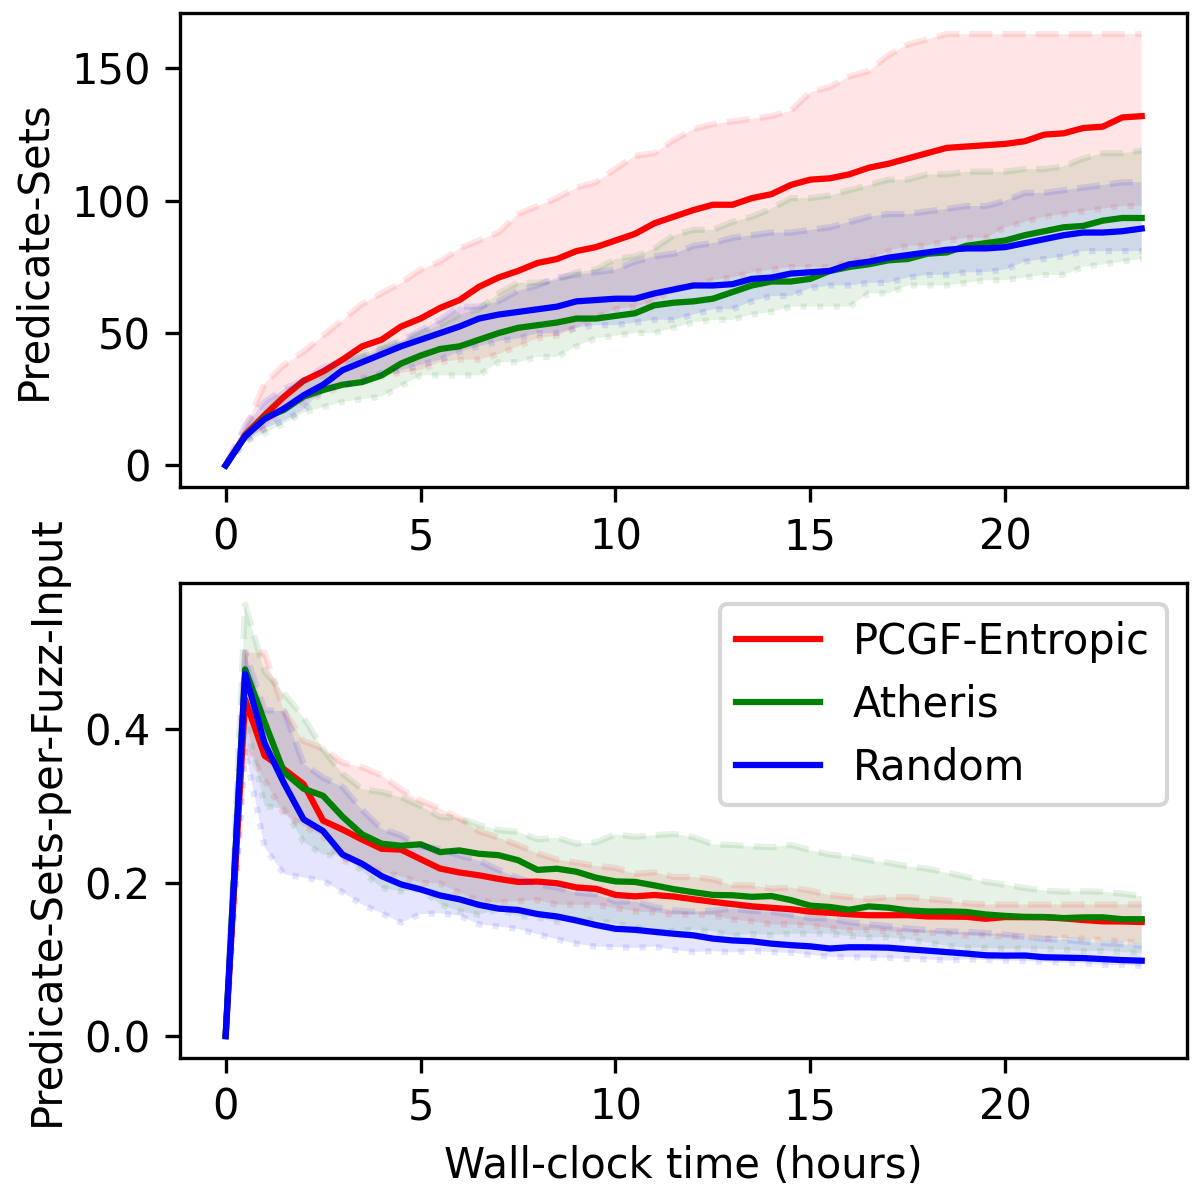
\includegraphics[width=0.6\linewidth]{figures/chapter5/RQ1/(PCGF-Entropic,Atheris,Random)_TFPP_all-coverage_(Predicate-Sets,Predicate-Sets-per-Fuzz-Input).png}
    \caption{RQ1, TF++ agent.}
    \label{fig:RQ1-TFPP}
\end{figure}

\begin{figure}
    \centering
    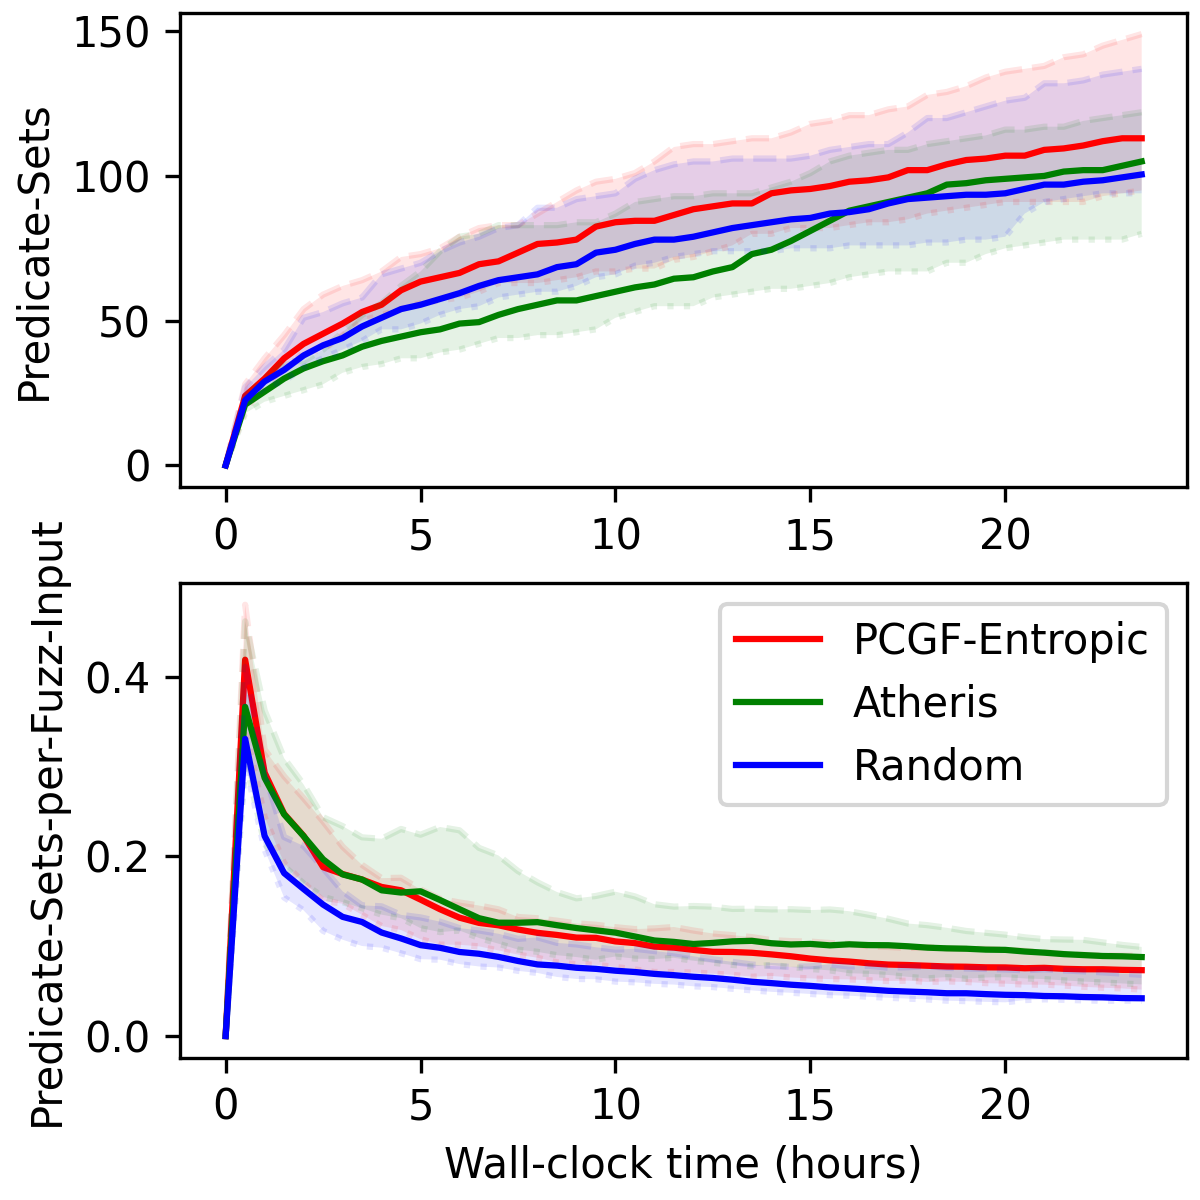
\includegraphics[width=0.6\linewidth]{figures/chapter5/RQ1/(PCGF-Entropic,Atheris,Random)_autopilot_all-coverage_(Predicate-Sets,Predicate-Sets-per-Fuzz-Input).png}
    \caption{RQ1, CARLA autopilot agent.}
    \label{fig:RQ1-autopilot}
\end{figure}

\begin{figure}
    \centering
    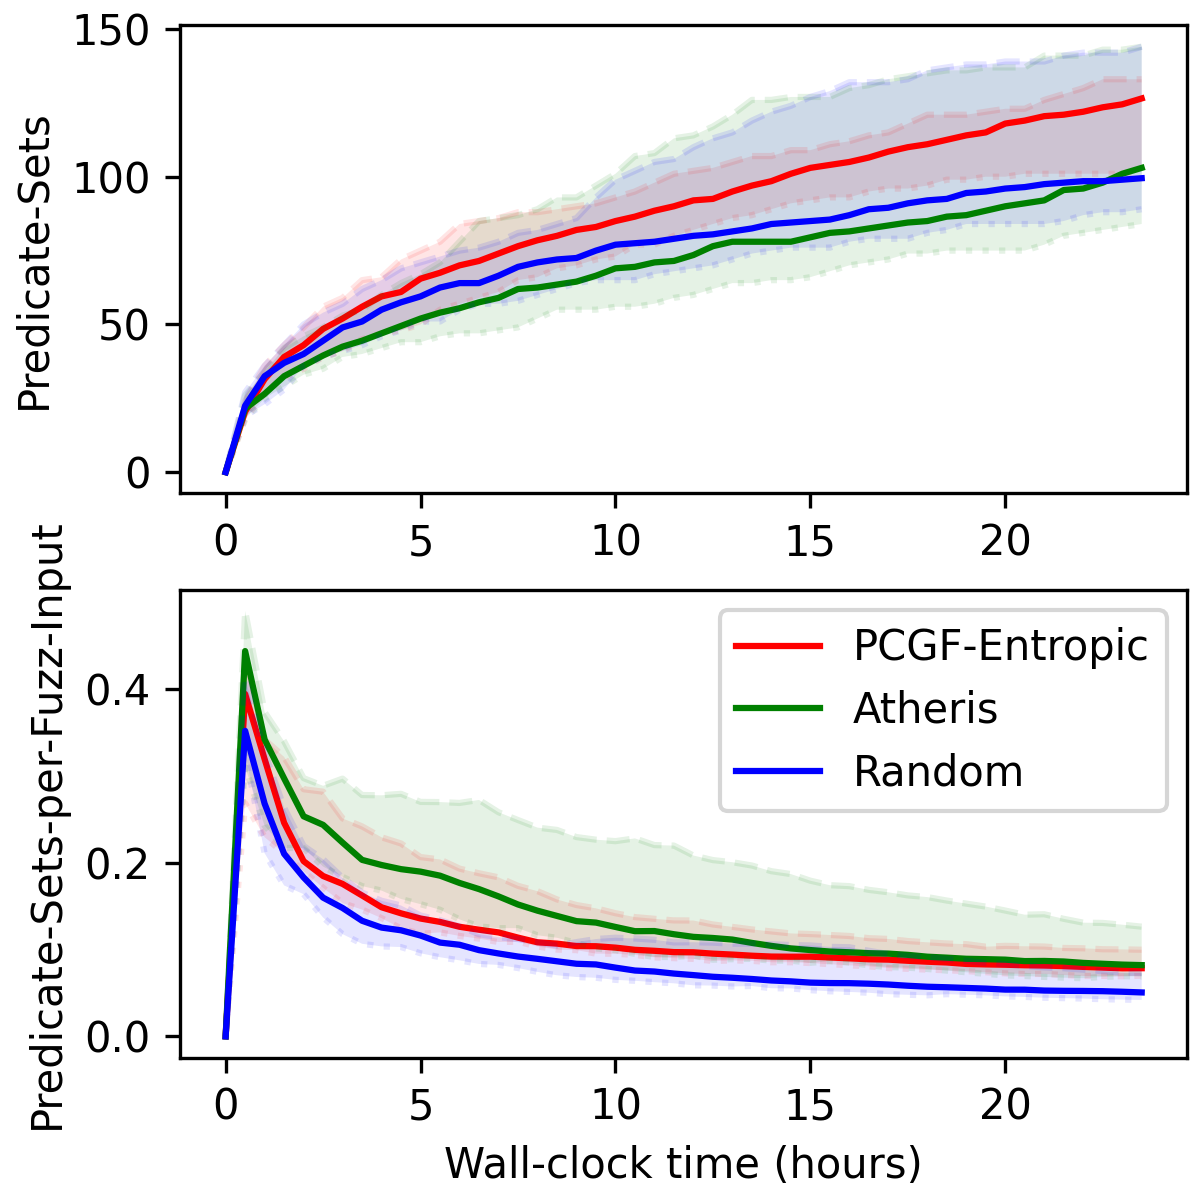
\includegraphics[width=0.6\linewidth]{figures/chapter5/RQ1/(PCGF-Entropic,Atheris,Random)_BehaviorAgent_all-coverage_(Predicate-Sets,Predicate-Sets-per-Fuzz-Input).png}
    \caption{RQ1, CARLA BehaviorAgent agent.}
    \label{fig:RQ1-BehaviorAgent}
\end{figure}

\begin{figure}
    \centering
    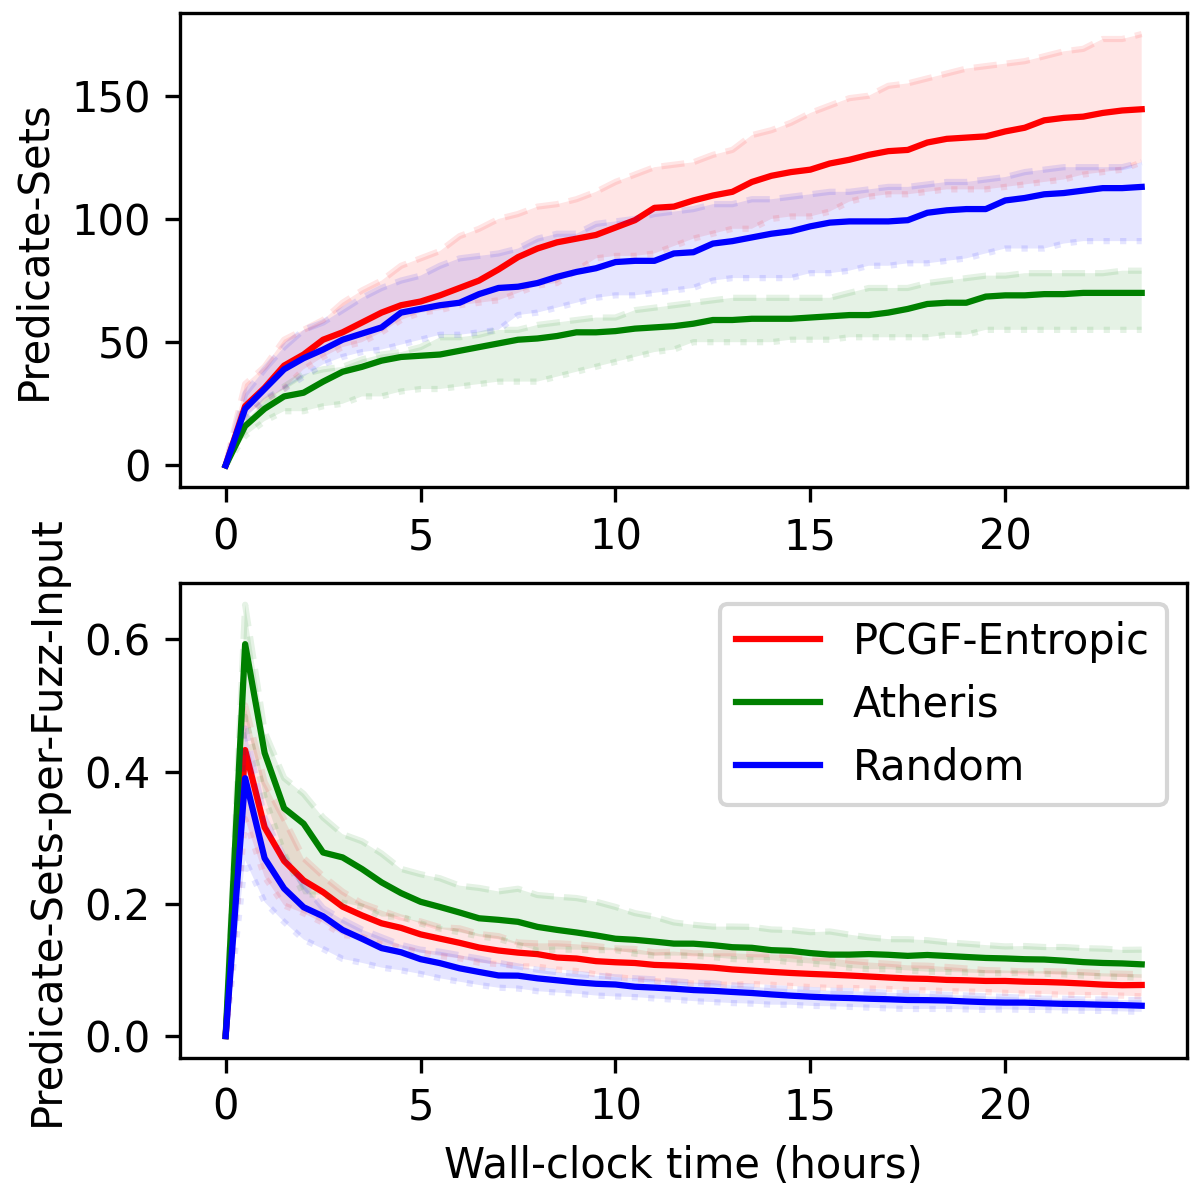
\includegraphics[width=0.6\linewidth]{figures/chapter5/RQ1/(PCGF-Entropic,Atheris,Random)_intersectionAgent_all-coverage_(Predicate-Sets,Predicate-Sets-per-Fuzz-Input).png}
    \caption{RQ1, SCENIC agent.}
    \label{fig:RQ1-SCENIC}
\end{figure}




%---------------------
\subsubsection{Results}

Our coverage criterion is to increase the cumulative number of unique predicate evaluations.
% 
Furthermore, it is desirable to achieve this coverage in as few test scenarios as possible.
% 
The evolution of coverage metrics over time and the coverage improvement per valid fuzz input for all the techniques for each agent are provided in Figures~\ref{fig:RQ1-TFPP},\ref{fig:RQ1-autopilot},\ref{fig:RQ1-BehaviorAgent},\ref{fig:RQ1-SCENIC}.
% 
In each figure, the different techniques are color coded; the solid curve shows the median coverage of all the trials and the bank around it shows the range, i.e., the minimum and maximum coverage obtained by each trial.
% 
The minimum coverage trial is dotted, and the maximum coverage trial is dashed.




We would like to highlight a few important aspects of the results.
% 
First is that the predicate coverage guided fuzzer that implements the Entropic power schedule (PCGF-Entropic) outperforms both the random fuzzer and Atheris irrespective of the AV agent under test.
% 
This observation is not surprising since a custom fuzzer to improve a specific metric is expected to improve the metric.
% 
However, we emphasize that the coverage obtained by PCGF is better than random and Atheris for any amount of computation budget allocated to it for a wide variety of AV agents.


Second, while random fuzzer achieves the same coverage as Atheris for most agents, it generates a lot more test-case instances.
% 
This is because the computational resources required to generate a new input using randomization is very low, as a result, it generates several test instances.
%
This difference gets amplified in the case of the SCENIC agent since SCENIC's NewtonianSimulator does not need heavy computational resources e.g. for rendering graphics.
% 
Therefore, if one considers the coverage-per-fuzz-input metric, random fuzzer always performs worse than the other two.


\begin{table}[]
    \centering
\begin{tabular}{|c|c|c|c|}
\hline
 & Random & Atheris & PCGF-Entropic\\
\hline
TF++ & 92, 920 & 97, 670 & 132, 929 \\
BehaviorAgent & 108, 2088 & 104, 1241 & 124, 1553 \\
AutoPilot & 107, 2400 & 104, 1298 & 118, 1692 \\
Scenic agent & 112, 2589 & 70, 668 & 150, 2009 \\
% Old numbers with violations.
% TF++ & 92, 920, 8 & 97, 670, 7 & 132, 929, 8\\
% BehaviorAgent & 108, 2088, 12 & 104, 1241, 12 & 124, 1553, 14\\
% AutoPilot & 107, 2400, 7 & 104, 1298, 8 & 118, 1692, 8\\
% Scenic agent & 112, 2589, 4 & 70, 668, 3 & 150, 2009,5\\
\hline
\end{tabular}
    \caption{Table documenting the performance of different fuzzing techniques on different AV agents. Each cell contains the median coverage obtained by the techniques and the total number of valid fuzz inputs generated.}
    \label{tab:all-medians}
\end{table}

Table~\ref{tab:all-medians} summarizes the median coverage and the median number of valid fuzz inputs generated for a given fuzzing technique on a given agent.
% 
% We calculate the unique set of predicates covered as the predicates that are covered by this technique but were not covered by the other two.
% 
From Table~\ref{tab:all-medians}, it is clear that PCGF-Entropic is simple enough to generate several valid fuzz inputs, but also mutates the vehicles behaviors in sufficiently complex ways to improve coverage.
% 
While Table~\ref{tab:all-medians} quantifies the benefits of using predicate coverage guided fuzzer, the temporal evolution of the number of fuzz inputs highlights that for any computation budget, the coverage-guided fuzzer returns a better coverage.
 

